% lintrans - The linear transformation visualizer
% Copyright (C) 2021-2022 D. Dyson (DoctorDalek1963)

% This program is licensed under GNU GPLv3, available here:
% <https://www.gnu.org/licenses/gpl-3.0.html>

\documentclass[../development.tex]{subfiles}

\begin{document}

\subsubsection{Fixing slots and signals\label{development:preparing-for-v0.2.1:fixing-slots-and-signals}}

I was perusing the Qt5 documentation when I learned about the difference between the \pyinline{dialog.finished} signal and the \pyinline{dialog.accepted} signal. I decided to rework some old code to make better use these signals.

When defining a new matrix or dialog settings, we only want to save the new data if the user actually accepted the dialog by clicking the confirm button. We don't want to save it if they clicked cancel. However, in the case of the error message dialog, we always want to update the render buttons when it's closed, no matter how the user closed the dialog.

%: 66242465222a153a5f37c4a1a3c2bd50bfd90933
%: src/lintrans/gui/main_window.py:35,447-448,461-469,478-483,493,511-512 noscopes

I also added the \pyinline{@pyqtSlot()} decorator to all the relevant methods in the matrix definition dialogs. The types in the brackets indicate the signature of the method.

A slot in Qt5 is just a method that is expected to be connected to a signal, so it gets called from the event loop. Using the decorator makes it clear that a method is a slot, and also allows slightly better performance.

%: 9beff9cf25d3af655e134205572a5668279f42cc
%: src/lintrans/gui/dialogs/define_new_matrix.py:67,138-140,143-144,155-157,164,194-195,203-204,214-215,226,276-277,288-289,305-306,317,348-349,356-357,364-365 noscopes

\subsubsection{Linking in documentation\label{development:preparing-for-v0.2.1:linking-in-documentation}}

I've been using Sphinx\cite{sphinx} for my documentation this whole time, and I've been using the Sphinx extension \texttt{intersphinx} to link to the Python standard library documentation. It uses a system of binary inventory files which define a reference map between names to use in the documentation, and where to link those names to. I recently learned of the \texttt{sphobjinv} Python package, which allows you to easily create your own local inventory files to reference some external source of documentation, such as the Qt5 documentation. I read through the \texttt{sphobjinv} documentation\cite{sphobjinv-2.2-docs} and designed a small script to read a custom text file, and create the binary inventory file needed by Sphinx.

%: 5455265a51666e29ab976152c1a758a422e1004a
%: docs/create_objects_inv.py:9-64

Line 11 should say \enquote{must have .html suffices}.

%: aab8e88b0e2cdae8038c9935031c74bcdae0ad5c
%: docs/pyqt5-objects.txt language="lexers.py:SphObjInvTextLexer -x"

I then just had to change all the references to Qt5 things in the documentation and then Sphinx would automatically link all the Qt5 references to their appropriate links, as defined in this file.

\subsubsection{Improving tests\label{development:preparing-for-v0.2.1:improving-tests}}

I made some small improvements to the unit tests by making sure they handled greedy index parsing, which means that something like \texttt{A\textasciicircum2 3B} will get parsed as \texttt{A\textasciicircum\{23\}B} because whitespace is ignored, as well asserting that all invalid expressions raise \pyinline{MatrixParseError}. I also added the copyright comment to the test files.

This was a tiny change, but worth noting.

%: c07d97024e1fe00ab110f43e5c7e6737c955d680
%: tests/matrices/test_parse_and_validate_expression.py:41,50-51,55,72-73,75,78-83

%: 70e1a7271a61f3009cc4d342f46743b248498a1c
%: tests/matrices/test_parse_and_validate_expression.py:26-31,86-90

\pytestScreenshot{70e1a7271a61f3009cc4d342f46743b248498a1c}

\subsubsection{The Windows version file\label{development:preparing-for-v0.2.1:the-windows-version-file}}

Windows stores metadata for \texttt{.exe} files inside the \texttt{.exe} files themselves\cite{msdocs-version-information-structures}\cite{msdocs-versioninfo-resource}. PyInstaller lets you embed that metadata when compiling on Windows, using a version file\cite{pyintaller-4.10-capturing-windows-version-data}. Obviously, I wanted to include this metadata in my compiled \texttt{.exe} in the release.

I created a simple \texttt{precompile.py} script that would create different pre-compilation artefacts. I could then use these in the compilation workflow for GitHub Actions. I started with just Windows, but obviously I'm going to expand into Linux and macOS as well later.

%: 2126959cb6f836b1bc6c92dad859b43cbd86e1ab
%: precompile.py:9-103

%: 2126959cb6f836b1bc6c92dad859b43cbd86e1ab
%: .github/workflows/compile-release.yaml:8,60,68,87-104 noscopes language=yaml

I quickly realised that this design would make the compilation process more complicated, since the process would be in separate parts. Instead, I decided to create a unified compilation script, which runs a pre-compile step dependent on the operating system, and then compiles the program with the \pyinline{PyInstaller.__main__.run()} function.

%: ca674c7f7d61e8eed3410d456787cfe5b2bc28e5
%: compile.py:9-180

This new compilation script captures the whole process. On Linux or macOS, it just compiles the program with PyInstaller. On Windows, it has to generate the version file, then compile the program with an additional argument to include the version file. I then updated the GitHub Actions workflow to use this new compilation script.

%: e47fe732954bf018128bdcb5ee9c354910517f36
%: .github/workflows/compile-release.yaml:8,60,68,87-88 noscopes language=yaml

\subsubsection{Compiling for macOS\label{development:preparing-for-v0.2.1:compiling-for-macos}}

Compiling for macOS is considerably more difficult. I run Ubuntu as my primary operating system. I used to use Windows and I have a Windows 10 virtual machine, so compiling for Windows was never an issue. But I've never used a Mac, and Apple don't like people installing macOS on non-Apple hardware. Getting a virtual machine set up running macOS Monterey was quite difficult, but I eventually managed to get it working somewhat properly.

Once I had \texttt{lintrans} compiling on macOS, I wanted to do something similar to what I did with Windows, where I added extra metadata to the executable. In macOS, executables are bundled as \texttt{.app} files, which are just directory structures, containing the necessary files and metadata\cite{apple-bundle-structures}. All the metadata for an application bundle is contained in the \texttt{Info.plist} file in the bundle\cite{apple-about-info.plist-files}\cite{apple-about-info.plist-keys-and-values}. After reading the documentation for these files, I created one for \texttt{lintrans}.

%: e716000521c92259ed4a1b33ab37e3860a7b7875
%: compile.py:92-134,149-155

This could would automatically generate the \texttt{Info.plist} file and write it to the correct place. However, I couldn't distribute this bundled app, since Apple requires an app to be signed by a trusted author before other people can download and run that code on their own Apple devices\cite{apple-about-code-signing}. And unfortunately, Apple charges \$99 per year for membership to their \enquote{Apple Developer Program}, which is required to become a trusted developer\cite{apple-developer-program-enrollment}\footnote{The price is listed in the small print at the bottom of the page.}.

Microsoft also wants its developers to sign their code for security and trust, and also charges for this privilege. But on Windows, you can run a foreign, unsigned app so long as you dismiss the potential virus warning. On macOS, it's completely forbidden.

I don't particularly want to pay \$99 per year to compile \texttt{lintrans} for macOS, when my audience on that platform is realistically almost zero, so I just removed macOS from the GitHub Actions publish workflow. For anyone that wants to run \texttt{lintrans} on macOS, I will provide instructions to compile it from source, since I can't distribute a binary file that I built myself. I will however continue to run the unit tests and compile the program on macOS in GitHub Actions, to ensure that everything works fine on that platform.

\subsubsection{Supporting flags\label{development:preparing-for-v0.2.1:supporting-flags}}

Most Linux apps support command line arguments and/or flags\footnote{For explanation and examples, see \url{https://betterdev.blog/command-line-arguments-anatomy-explained/}}, and so I wanted to support these with \texttt{lintrans}. I wanted one flag to display help for the program, and one flag to display the version number of the program. Implementing this was very simple and I didn't bother using a library like \texttt{argparse}; I just used \pyinline{sys.argv}.

%: ffc603f1bf049811cb927f879ce7989456f6a537
%: src/lintrans/__main__.py:9-55

Here is the expected output when using these flags at a shell prompt:

\begin{minted}[linenos=false]{console}
$ python -m lintrans --help
Usage: /home/dyson/repos/lintrans/src/lintrans/__main__.py [option]

Options:
    -h, --help       Display this help text and exit
    -V, --version    Display the version information and exit

Any other options will get passed to the QApplication constructor.
If you don't know what that means, then don't provide any arguments and just the run the program.
$ python -m lintrans --version
lintrans (version 0.2.0)
The linear transformation visualizer

Copyright (C) 2021-2022 D. Dyson (DoctorDalek1963)

This program is licensed under GNU GPLv3, available here:
<https://www.gnu.org/licenses/gpl-3.0.html>
\end{minted}

\subsubsection{Adding the about dialog\label{development:preparing-for-v0.2.1:adding-the-about-dialog}}

In addition to the help and version information available from the command line, most apps with a GUI provide a graphical way to access information about the app, typically in the form of an about box. I wanted to do this for \texttt{lintrans}. I had intended to have this from the start, but it now felt like the right time to implement it, since I was preparing to release version \texttt{0.2.1}.

To do this, I create a new file to house the new dialog class, and then added the functionality to the original button, so that it would now open the new dialog.

%: 7423fff72f09b5f5a3253c734d42c4e7c3182efe
%: src/lintrans/gui/dialogs/misc.py

%: 7423fff72f09b5f5a3253c734d42c4e7c3182efe
%: src/lintrans/gui/main_window.py:64-65,97-99,117

This feature works just as expected.

\begin{figure}[H]
	\centering
	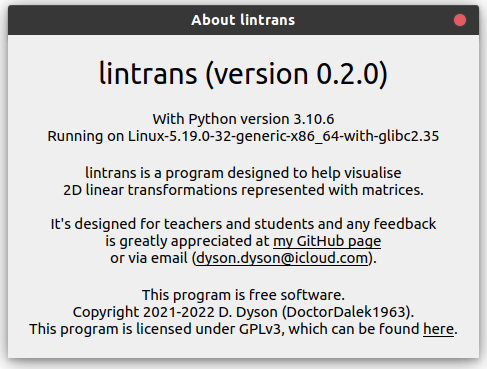
\includegraphics[width=0.8\linewidth]{development/7423fff72f09b5f5a3253c734d42c4e7c3182efe/about-dialog.png}
	\caption{The about dialog}
	\label{fig:development:7423fff72f09b5f5a3253c734d42c4e7c3182efe:about-dialog.png}
\end{figure}

\subsubsection{Creating the \texttt{FixedSizeDialog} class\label{development:preparing-for-v0.2.1:creating-the-FixedSizeDialog-class}}

Currently, several dialogs are a fixed size, meaning they can't be resized. Qt5 doesn't have the option to make a dialog non-resizeable - that's only available for whole windows - so to achieve this effect, I had to add the line \pyinline{self.setFixedSize(self.baseSize())} to the end of the constructor for every fixed size dialog\footnote{This works because Qt5 needs to arrange all the widgets and allocate space for all of them first, and then we can use that calculated size as the fixed size.}. This was easy to forget and it didn't make it immediately clear which dialogs were fixed size and which weren't.

To fix this, I decided to use a different technique, by overriding the \pyinline{open()} method of the dialog. This method gets called when the dialog is first opened. If I called the superclass' implementation first to do all the actual opening logic, then I could use that same previous technique to set the fixed size to whatever Qt5 had calculated it to be. By overriding a method, I could put that override into a simple superclass called \pyinline{FixedSizeDialog} and then make all fixed size dialogs inherit from this class instead of just \pyinline{QDialog}.

%: a59ea87fb37fc593cf0bae3066bdbd24be656798
%: src/lintrans/gui/dialogs/misc.py:20-29,32

%: a59ea87fb37fc593cf0bae3066bdbd24be656798
%: src/lintrans/gui/dialogs/define_new_matrix.py:68

%: a59ea87fb37fc593cf0bae3066bdbd24be656798
%: src/lintrans/gui/dialogs/settings.py:21

I used \pyinline{self.size()} here instead of \pyinline{self.baseSize()} like before. There doesn't seem to be much difference, but the docs seem to suggest that \pyinline{self.size()} is more appropriate for this use case\cite{qt5-docs-qwidget-basesize}\cite{qt5-docs-qwidget-size}.

\subsubsection{Increasing minimum grid spacing\label{development:preparing-for-v0.2.1:increasing-minimum-grid-spacing}}

When you zoom out, the grid lines get closer and closer together. I previously limited this to 1 pixel, since the program would hang or crash if it was any lower. However, having the grid lines that close together made it very hard to see what was happening. I could easily fix this by limiting the minimum grid spacing to say, 5 pixels.

\begin{figure}[H]
	\centering
	\begin{minipage}{0.48\linewidth}
		\centering
		\includegraphics[width=\linewidth]{development/a59ea87fb37fc593cf0bae3066bdbd24be656798/zoomed-out.png}
		\caption{Fully zoomed out before}
		\label{fig:development:a59ea87fb37fc593cf0bae3066bdbd24be656798:zoomed-out.png}
	\end{minipage}\hfill
	\begin{minipage}{0.48\linewidth}
		\centering
		\includegraphics[width=\linewidth]{development/51d35018c81deaaf7e32646b1f99d6e46643bf24/zoomed-out.png}
		\caption{Fully zoomed out after}
		\label{fig:development:51d35018c81deaaf7e32646b1f99d6e46643bf24:zoomed-out.png}
	\end{minipage}
\end{figure}

%: 51d35018c81deaaf7e32646b1f99d6e46643bf24
%: src/lintrans/gui/plots/classes.py:39,154-166

\subsubsection{Creating a changelog\label{development:preparing-for-v0.2.1:creating-a-changelog}}

I've know about changelogs for a long time. They're used to keep track of changes to a project over time. I recently learned about the project \enquote{keep a changelog}, which tries to create a standard for changelog formats\cite{keep-a-changelog-1.0.0}. I want to have a proper changelog for lintrans, so I decided to implement one.

%: 47c68c7f4780d0e2c374cf12b9b54c031277af6d
%: CHANGELOG.md language="lexers.py:MarkdownWithCommentsLexer -x" comment="<!-- {} -->"

\subsubsection{Releasing \texttt{v0.2.1}\label{development:preparing-for-v0.2.1:releasing-v0.2.1}}

Now all I had to do for the release was update the version number in \texttt{__init__.py} and update the changelog to include the changes under the correct heading, and add a new, empty \enquote{Unreleased} heading.

%: d47f63eb0bcdc89cff5ed19afe2fc63899edf1d9
%: src/lintrans/__init__.py:13

%: d47f63eb0bcdc89cff5ed19afe2fc63899edf1d9
%: CHANGELOG.md language="lexers.py:MarkdownWithCommentsLexer -x" comment="<!-- {} -->"

\begin{figure}[H]
	\centering
	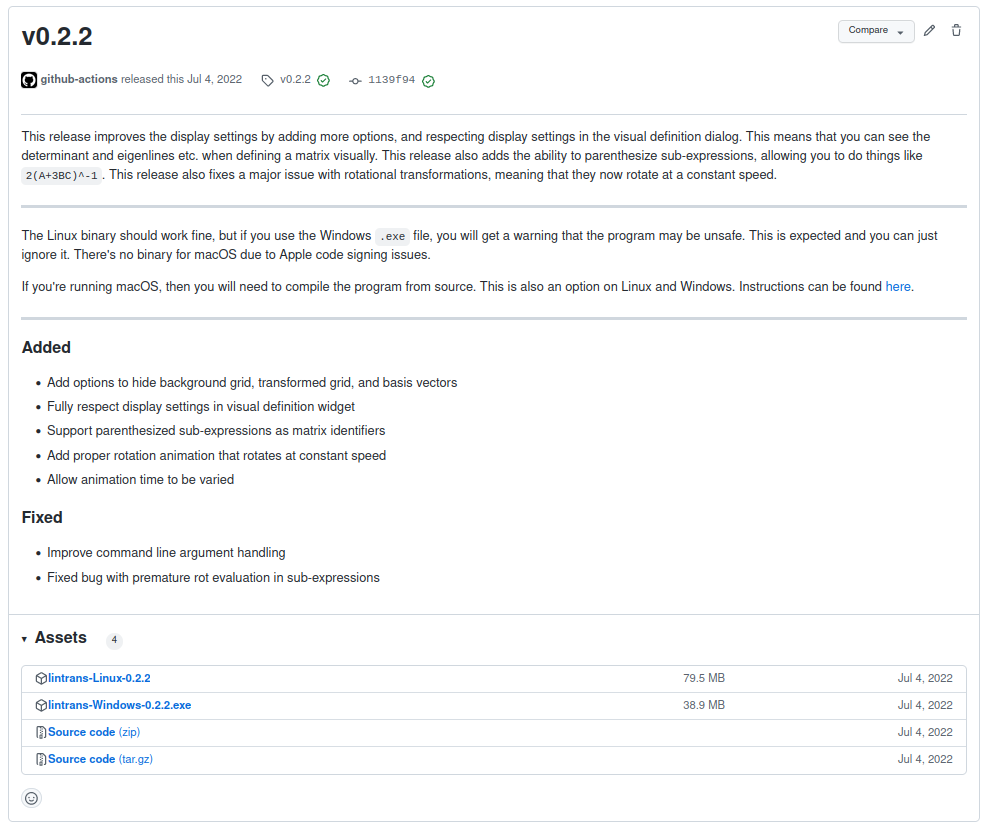
\includegraphics[width=0.8\linewidth]{development/d47f63eb0bcdc89cff5ed19afe2fc63899edf1d9/release.png}
	\caption{The release of \texttt{v0.2.1} on GitHub}
	\label{fig:development:d47f63eb0bcdc89cff5ed19afe2fc63899edf1d9:release.png}
\end{figure}

\subsubsection{Automating release note generation\label{development:preparing-for-v0.2.1:automating-release-note-generation}}

I had to copy the changelog over and polish up the release notes myself for this release. It would be quite convenient to have a script that does this automatically, so I made one.

%: 99a88575f9beb8fed2dcc41dacbb020b31bc8176
%: generate_release_notes.py

This script just parses the changelog and generates a file called \texttt{release_notes.md}, which I can then automatically use as the body for the GitHub release by changing the workflow.

%: 99a88575f9beb8fed2dcc41dacbb020b31bc8176
%: .github/workflows/compile-release.yaml:8,97,101,124-146 language=yaml

\end{document}
